\section{Bepaling E modulus}

We meten op analoge wijze het rekstrookje.
Dit is bij $R_a$ en $R_b$ gelijk aan $10\Omega$ en 
men bekomt dan de waarden in tabel \ref{tab:rekstrookje}.
\\ \\
Men heeft hier gekozen voor een type $A$ opstelling omdat
er aan de nodige voorwaarde voor type $A$ werd voldaan.

Voorwaarde type $A$ opstelling:
$$ R_A > R en R_B > R_x of R_A < R en R_B < R_x $$

\begin{table}[h]
    \centering
    \caption{Meetresultaten rekstrookje}
    \label{tab:rekstrookje}

    \begin{tabular}{| c | c | c | c | c |}
        \hline
        Kracht [N] & $R_{min} [\Omega]$& $R_{max} [\Omega]$& $I_{min}$ [mA] & $I_{max}$ [mA] \\ \hline
        0,981      & 130               & 120               & -0,041    & 0,003 \\ \hline
        1,962      & 130               & 120               &-0,047     & 0,003 \\ \hline
        2,943      & 130               & 120               &-0,04      & 0,004 \\ \hline
        3,924      & 130               & 120               &-0,04      & 0,004 \\ \hline
        4,905      & 130               & 120               &-0,039     & 0,004 \\ \hline
        5,886      & 130               & 120               &-0,039     & 0,004 \\ \hline
        6,867      & 130               & 120               &-0,038     & 0,005 \\ \hline
    \end{tabular}
\end{table}

\begin{figure}[h]
    \centering
    \caption{Lineaire interpolatie}
    \label{fig:lin_interpol_e}
    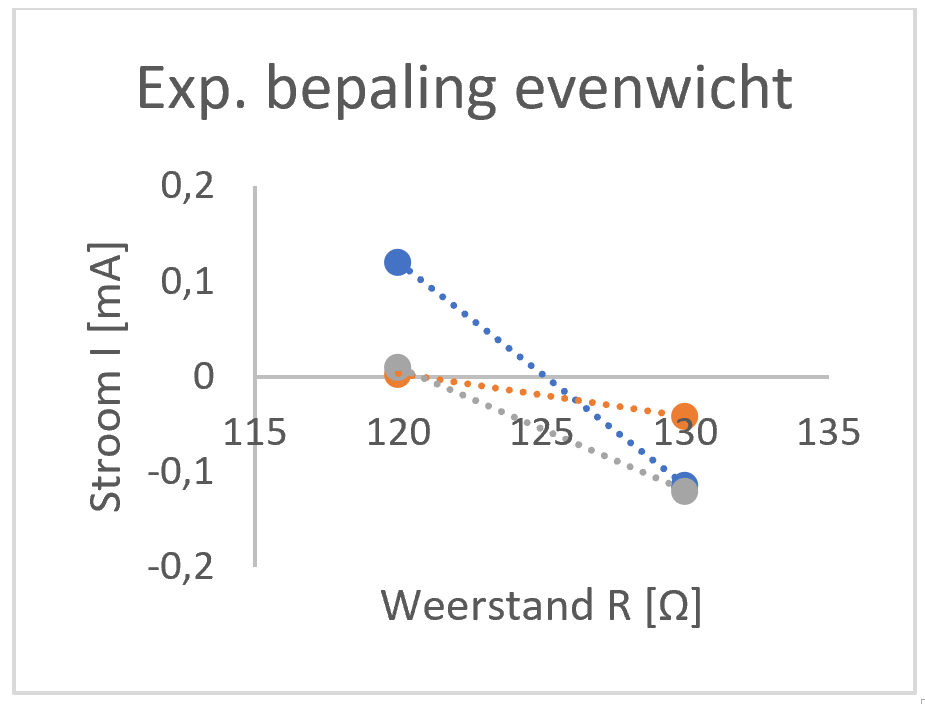
\includegraphics[width=0.7\textwidth]{img/tweede.png}
\end{figure}

Na interpolatie [\ref{fig:lin_interpol_e}] volgens volgende formule:

\begin{equation}
    R = R_{min} - \frac{\Delta R}{\Delta I} \cdot I_{min}
\end{equation}


bekomt men R. Met deze waarde wordt het mogelijk om $R_{x}$ te
berekenen via een schaalfactor 1 bepaald door $R_{a}$ en $R_{b}$.
\\

$\Delta R_{x}$ wordt dan weer bepaald door het verschil met de
nominale waarde van het rekstrookje (waarde van de weerstand
bij evenwicht, ongeveer $120\Omega$).
\\ \\
Men bekomt de waarden uit tabel \ref{tab:interpol_rekstrookje}

\begin{table}[h]
    \centering
    \caption{Interpolatie rekstrookje}
    \label{tab:interpol_rekstrookje}
    \begin{tabular}{| c | c | c | c |}
        \hline
        R [$\Omega$]    & Rx [$\Omega$] & $\Delta R_{x}$    & $\frac{\Delta R_{x}}{R_{x}}$ \\ \hline
        120,682         & 120,682       & 0,682             & 0,005650 \\ \hline
        120,600         & 120,600       & 0,600             & 0,004975 \\ \hline
        120,909         & 120,909       & 0,909             & 0,007519 \\ \hline
        120,909         & 120,909       & 0,909             & 0,007519 \\ \hline
        120,930         & 120,930       & 0,930             & 0,007692 \\ \hline
        120,930         & 120,930       & 0,930             & 0,007692 \\ \hline
        121,163         & 121,163       & 1,163             & 0,009597 \\ \hline
    \end{tabular}
\end{table}

Nu kan men een lineaire regressie uitvoeren met als x-waarden
de krachten uitgeoefend op het balkje en als y-waarden
$\frac{\Delta R_{x}}{R_{x}}$.

\begin{figure}[h]
    \centering
    \caption{Lineaire regressie $E$}
    \label{fig:lin_reg_E}
    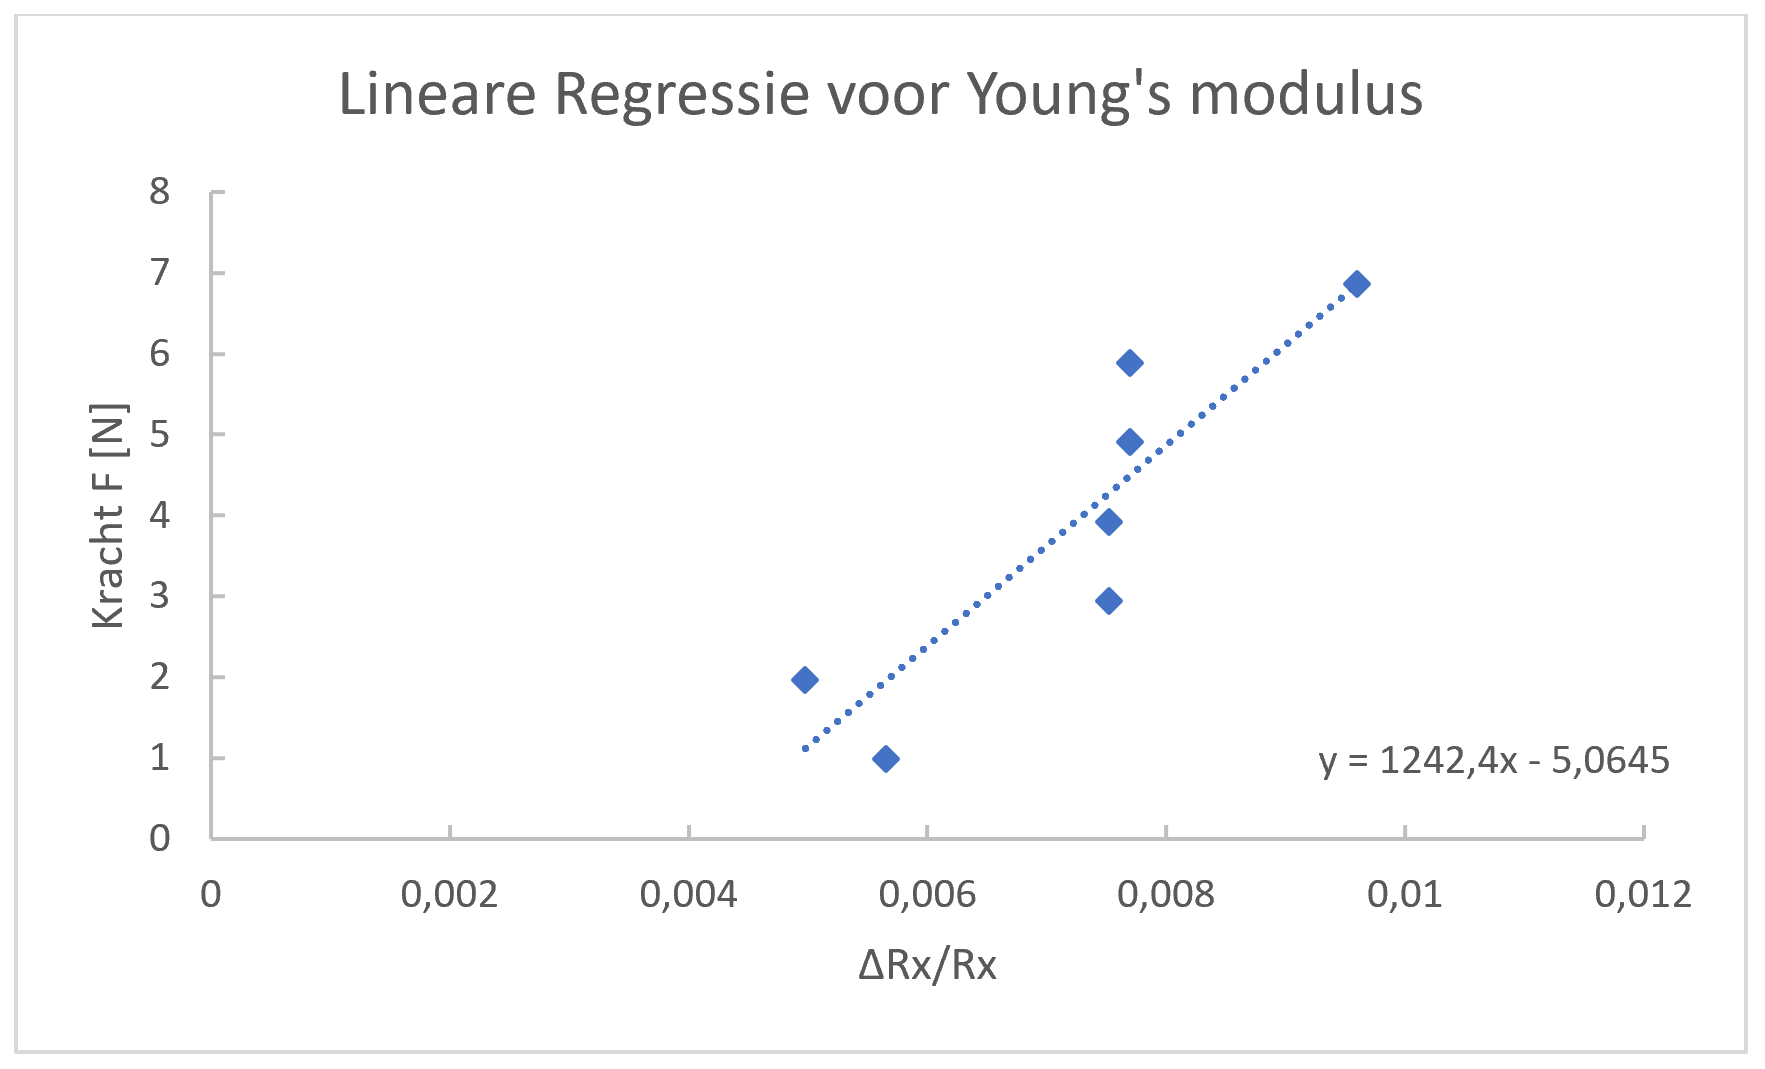
\includegraphics[width=0.7\textwidth]{img/grafiek.png}
\end{figure}

Met de lineaire regressie [\ref{fig:lin_reg_E}] functie in excel kan men nu de
richtingsco\"effici\"ent bepalen. Deze zal van volgende vorm
zijn:

\begin{equation}
    m = \frac{3}{2} \cdot \frac{K_1 \cdot L}{E \cdot b \cdot d^2}
\end{equation}

Na enige omvorming krijgt men een formule voor $E$:

\begin{equation}
    E = \frac{3}{2} \cdot \frac{K_1 \cdot L}{z \cdot b \cdot d^2}
\end{equation}

Samen met volgende fysische eigenschappen van het balkje:

\begin{table}[h]
    \centering
    \caption{Fysische eigenschappen balkje}
    \label{tab:fys_eig_balkje}
    \begin{tabular}{| c | c | c |}
        \hline
            & Waarde& Fout \\ \hline
        K1  & 2,110 & 0,01 \\ \hline
        L   & 0,250 & 0,00 \\ \hline
        b   & 0,020 & 0,00 \\ \hline
        d   & 0,005 & 0,00 \\ \hline
    \end{tabular}
\end{table}

Kan men nu $E$ en de fout hierop berekenen:

\begin{equation}
    E = 9,964E+09 \pm 4,7E+07
\end{equation}

\subsection{Bespreking resultaten}

Hoewel men hier een waarde uikomt ziet men dat de proeven
niet al te accuraat werden uitgevoerd. Dit kan liggen aan
de materiaalpech die men ervaarde tijdens het practicum. Ook
tijdstekort bezorgde extra druk waardoor er
onnauwkeurigheden gemakkelijk konden insluipen.

